\chapter{Killing 对称、体积与 Hodge 理论}

Levi--Civita 联络把度量与协变微分锁定在同一结构中以后，可以问两个彼此相关的问题。其一，哪些流保持度量，从而代表几何的连续对称？其二，度量如何把微分形式空间变成带内积的 Hilbert 型对象，使外微分 $\dd$ 拥有伴随算子并产生椭圆谱理论？前者引出 Killing 场，后者引出 Hodge 星、余微分与 Hodge 拉普拉斯算子。二者在同一处汇合：Killing 流保持由度量构造的一切自然算子，因此对称性可以与 Hodge 谱同时分解。

\section{Killing 场与测地线守恒量}

设 $(M,g)$ 为 Riemann 或 伪 Riemann 流形，$X$ 为光滑向量场。若其局部流 $\Phi_t$ 满足
\[
\Phi_t^*g=g,
\]
则称 $X$ 为 Killing 向量场。对 $t=0$ 求导，等价地写成
\begin{equation*}\boxed{\mathcal L_Xg=0.}
\end{equation*}
这个定义只表达“流保持度量”，尚未选坐标。使用 Levi--Civita 联络可以把它改写为一阶偏微分方程。

沿仿射参数测地线 $\gamma(s)$，令 $u=\dot\gamma$。Killing 场产生标量
\[
J_X:=g(X,u).
\]
利用 $\nabla_u u=0$ 与\eqnrefs{eq:math-dg-synthesis-killing-eq}，
\[
\begin{aligned}
\frac{\dd J_X}{\dd s}
&=g(\nabla_uX,u)+g(X,\nabla_uu)\\
&=\frac12(\mathcal L_Xg)(u,u)=0.
\end{aligned}
\]
因此
\begin{equation*}\boxed{\frac{\dd}{\dd s}g(X,\dot\gamma)=0.}
\end{equation*}
连续等距对称由此直接转化为测地线的一阶守恒量。

\begin{exbox}[Euclidean 平面的 Killing 代数]
在 $g=\dd x^2+\dd y^2$ 上写
\[
X=P(x,y)\partial_x+Q(x,y)\partial_y.
\]
Killing 方程化为
\[
\partial_xP=0,
\qquad
\partial_yQ=0,
\qquad
\partial_yP+\partial_xQ=0.
\]
故
\[
P=ay+b,
\qquad
Q=-ax+c,
\]
于是全部 Killing 场由
\[
\partial_x,
\qquad
\partial_y,
\qquad
y\partial_x-x\partial_y
\]
张成，分别对应两个平移与一个旋转。
\end{exbox}

\section{体积、Hodge 星与余微分}

若 $(M,g)$ 已定向，度量诱导体积形式。Riemann 情形局部写成
\begin{equation*}\operatorname{vol}_g
=\sqrt{\det(g_{ij})}\,
\dd x^1\wedge\cdots\wedge\dd x^n,
\end{equation*}
对 伪 Riemann 度量则将 $\det g$ 替换为 $|\det g|$。给定任意向量场 $X$，由于 $\mathcal L_X\operatorname{vol}_g$ 仍是顶次形式，存在唯一函数定义散度：
\begin{equation}\label{eq:math-dg-divergence-volume}
\mathcal L_X\operatorname{vol}_g=(\operatorname{div} X)\operatorname{vol}_g.
\end{equation}

由 Cartan 恒等式和顶次形式自动闭合 $\dd\operatorname{vol}_g=0$，
\[
\mathcal L_X\operatorname{vol}_g=\dd(\iota_{X}\operatorname{vol}_g).
\]
在坐标中展开可得
\begin{equation*}\boxed{
\operatorname{div} X
=\nabla_iX^i
=\frac{1}{\sqrt{|\det g|}}
\partial_i\!\left(\sqrt{|\det g|}\,X^i\right).}
\end{equation*}

Killing 方程取迹得到
\[
2\nabla_iX^i=0,
\]
因此 Killing 场满足
\begin{equation*}\operatorname{div} X=0,
\qquad
\mathcal L_X\operatorname{vol}_g=0.
\end{equation*}
等距流不仅保持长度和角度，也保持由同一度量诱导的体积。

从体积形式继续到微分形式的度量对偶。Hodge 星把同一度量对体积与内积的作用统一起来，并自然导出余微分与 Hodge 拉普拉斯算子。

从这里起假设 $(M,g)$ 为定向 Riemann 流形。度量在 $k$-形式上诱导点态内积 $\langle\cdot,\cdot\rangle_g$。Hodge 星算子
\begin{equation*}*:\Omega^k(M)\to\Omega^{n-k}(M)
\end{equation*}
由
\begin{equation}\label{eq:math-dg-hodge-star-characterization}
\alpha\wedge *\beta
=\langle\alpha,\beta\rangle_g\,\operatorname{vol}_g
\end{equation}
唯一确定。对 Riemann 度量，
\[
**\alpha=(-1)^{k(n-k)}\alpha.
\]
因此 $*$ 不是额外选择，而是“度量 + 定向”在外代数上的自然延伸。

在紧支撑形式上定义 $L^2$ 内积
\[
(\alpha,\beta)_{L^2}
:=\int_M\alpha\wedge *\beta.
\]
外微分的形式伴随称为余微分。对 $k$-形式采用约定
\begin{equation*}\delta
:=(-1)^{n(k+1)+1}*\dd*:
\Omega^k(M)\to\Omega^{k-1}(M).
\end{equation*}
若流形无边界，或形式满足足以消去边界项的条件，则 Stokes 定理给出
\[
(\dd\alpha,\beta)_{L^2}
=(\alpha,\delta\beta)_{L^2}.
\]
特别地，对向量场 $X$ 的对偶一形式 $X^\flat$，
\begin{equation*}\boxed{\operatorname{div} X=-\delta X^\flat=*\dd*X^\flat.}
\end{equation*}
最后一个等号使用的是 $k=1$ 时 $\delta=-*\dd*$。这一定号关系必须与\eqnrefs{eq:math-dg-divergence-volume}一致；若把 $-*\dd*X^\flat$ 直接写成散度，会与当前余微分约定差一个负号。

Hodge--de Rham 拉普拉斯算子 定义为
\begin{equation*}\Delta:=\dd\delta+\delta\dd.
\end{equation*}
它保持形式次数。对任意紧支撑 $k$-形式，
\begin{equation}\label{eq:math-dg-hodge-energy}
(\alpha,\Delta\alpha)_{L^2}
=\|\dd\alpha\|_{L^2}^2+\|\delta\alpha\|_{L^2}^2\ge0.
\end{equation}
因此在无边界紧致 Riemann 流形上，$\Delta$ 是非负自伴椭圆算子；这一点把本章与前面的谱理论直接接起来。

Hodge 拉普拉斯算子 的主符号恰为 $|\xi|_g^2$（\eqnrefs{eq:math-dg-hodge-principal-symbol}），这是其椭圆性与谱离散性的来源。

\section{Hodge 分解与上同调}

记
\[
\mathcal H^k(M):=\ker\Delta\big|_{\Omega^k(M)}
\]
为 调和 $k$-形式空间。由\eqnrefs{eq:math-dg-hodge-energy}，
\begin{equation}\label{eq:math-dg-harmonic-closed-coclosed}
\Delta\alpha=0
\quad\Longleftrightarrow\quad
\dd\alpha=0,
\ \delta\alpha=0.
\end{equation}

\begin{theorem}[紧致无边界流形上的 Hodge 分解]\label{thm:math-dg-hodge-decomposition}
设 $(M,g)$ 为紧致、定向、无边界 Riemann 流形。则任意 $\alpha\in\Omega^k(M)$ 都有正交分解
\begin{equation}\label{eq:math-dg-hodge-decomposition}
\boxed{
\alpha=\dd\beta+\delta\gamma+\alpha_{\mathcal H},
\qquad
\alpha_{\mathcal H}\in\mathcal H^k(M).}
\end{equation}
其中 精确、coexact 与 调和 三个分量作为形式是唯一的；势 $\beta$ 与 $\gamma$ 本身一般不唯一。并且自然映射
\begin{equation*}\mathcal H^k(M)\longrightarrow H_{\mathrm{dR}}^k(M),
\qquad
\eta\longmapsto[\eta]
\end{equation*}
是线性同构。
\end{theorem}


\par
\begin{workedexample}
设 \(M\) 为紧致定向无边界 Riemann 流形。若闭形式 \(\alpha\) 的 Hodge 分解为
\[
\alpha=\dd\beta+\delta\gamma+\alpha_{\mathcal H},
\]
不用直接引用正文结论，证明 \(\delta\gamma=0\)，从而说明 \([\alpha]=[\alpha_{\mathcal H}]\)。再说明为什么 调和 分量 \(\alpha_{\mathcal H}\) 唯一而 \(\beta\) 不必唯一。
\textbf{解。} 对分解取外微分，因 \(d\alpha=0\)、\(d^2\beta=0\) 且调和形式闭，得 \(d\delta\gamma=0\)。由 \(\delta\) 与 \(d\) 在无边界紧流形上的伴随关系，
\[
\|\delta\gamma\|^2=\langle\delta\gamma,\delta\gamma\rangle
=\langle\gamma,d\delta\gamma\rangle=0,
\]
所以 \(\delta\gamma=0\)，并有 \(\alpha=d\beta+\alpha_{\mathcal H}\)，两者同属一个上同调类。若两个调和形式代表同一类，其差既调和又恰当，故范数平方为零，代表元唯一；但 \(\beta\) 可加任意闭 \((k-1)\)-形式而不改变 \(d\beta\)，故不必唯一。
\end{workedexample}
\par

意义：Hodge 分解 $\Omega^k=\dd\Omega^{k-1}\oplus\delta\Omega^{k+1}\oplus\mathcal H^k$ 把任意微分形式正交分解为恰当、余恰当和调和三部分。每个 de Rham 上同调类有且仅有一个调和代表元——这使得上同调（拓扑不变量）可用调和形式（分析对象）实现。实例：紧曲面 $\Sigma_g$ 上，$H^1_{\mathrm{dR}}$ 由 $2g$ 个线性无关的调和 1-形式张成，对应 $g$ 个环柄的经线和纬线方向。在物理中，Maxwell 方程 $\dd F=0$、$\delta F=J$ 的解存在性恰好由 Hodge 分解保证：$F=F_{\mathcal H}+\dd A+\delta B$，规范势 $A$ 存在当且仅当 $[F]\in H^2$ 被源 $J$ 的约束允许。

Hodge 定理还把一个纯拓扑结论变成了几乎一行的 $L^2$ 论证。设 $M$ 为紧致、定向、无边界 $n$ 维流形。Hodge 星给出
\[
*:\Omega^k(M)\longrightarrow\Omega^{n-k}(M),
\]
并与 Hodge 拉普拉斯算子 对易：
\[
\Delta_H(*\alpha)=*(\Delta_H\alpha).
\]
因此 $*$ 限制为 调和 空间之间的同构
\begin{equation}
*:\mathcal H^k(M)\overset{\sim}{\longrightarrow}\mathcal H^{n-k}(M).
\label{eq:math-dg-hodge-star-harmonic-isomorphism}
\end{equation}
结合 Hodge--de Rham 同构，就得到 Poincaré 对偶 的解析实现。

\begin{theorem}[Poincaré 对偶的 Hodge 实现]\label{thm:math-dg-poincare-duality-hodge}
对紧致、定向、无边界 $n$ 维流形 $M$，配对
\begin{equation}
H^k_{\mathrm{dR}}(M)\times H^{n-k}_{\mathrm{dR}}(M)
\longrightarrow\RR,
\qquad
([\alpha],[\beta])\longmapsto\int_M\alpha\wedge\beta
\label{eq:math-dg-poincare-pairing}
\end{equation}
是非退化的。特别地，
\[
b_k(M)=b_{n-k}(M).
\]
\end{theorem}

这个证明说明定向、紧致和无边界三个条件分别在何处进入：定向保证可全局积分顶次形式；紧致保证积分与 调和 空间的有限维谱理论良好；无边界使 Stokes 边界项消失。若有边界，正确对象会变成 绝对/相对 上同调之间的 Lefschetz 对偶，正好与后面的两类 Hodge 边界条件对应。
Hodge 拉普拉斯算子 的定义使用外微分与余微分，而 Riemann 几何中还存在由 Levi--Civita 联络构造的 rough 拉普拉斯算子
\[
\nabla^*\nabla:
\Omega^k(M)\to\Omega^k(M).
\]
二者具有相同的二阶主符号，因此差只能是零阶曲率作用。一般 Weitzenböck 公式写成
\begin{equation*}\boxed{
\Delta_H
=\nabla^*\nabla+\mathcal R_k
},\end{equation*}
其中 $\mathcal R_k$ 是 Riemann 曲率在 $k$-形式表示上的代数作用。对 $0$-形式，$\mathcal R_0=0$；对 $1$-形式最简单：
\begin{equation}
\boxed{
(\Delta_H\alpha)_i
=(\nabla^*\nabla\alpha)_i
+\operatorname{Ric}_i{}^j\alpha_j
}.
\label{eq:math-dg-weitzenbock-oneform}
\end{equation}
这条公式把拓扑信息、椭圆 PDE 与 Ricci 曲率直接连接起来。

若 $M$ 紧致无边界且 $\alpha$ 为 调和 $1$-形式，则
\[
0=(\alpha,\Delta_H\alpha)
=\|\nabla\alpha\|_{L^2}^2
+\int_M\operatorname{Ric}(\alpha^\sharp,\alpha^\sharp)\,\operatorname{vol}_g.
\]
若 $\operatorname{Ric}>0$ 处处正定，两项都非负且第二项只有 $\alpha=0$ 才能消失，因此
\[
\mathcal H^1(M)=0,
\qquad
H^1_{\mathrm{dR}}(M)=0.
\]
这就是最基本的 Bochner vanishing 定理：曲率的正性通过 Weitzenböck 零阶项排除 调和 代表元，从而杀掉上同调。

Bochner 方法还给出一个比“$H^1$ 消失”更定量的结论。对函数 $f$，采用本书非负 拉普拉斯算子 约定
\[
\Delta f=-\nabla^i\nabla_i f,
\]
Bochner 恒等式可写成
\begin{equation}
\frac12\Delta|\nabla f|^2
=\langle\nabla f,\nabla\Delta f\rangle
-|\nabla^2f|^2
-\operatorname{Ric}(\nabla f,\nabla f).
\label{eq:math-dg-bochner-function}
\end{equation}
若 $M$ 紧致且 $\operatorname{Ric}\ge(n-1)k g$，$k>0$，对第一非零本征函数
\[
\Delta f=\lambda_1 f,
\qquad
\int_M f\,\operatorname{vol}_g=0,
\]
积分\eqnrefs{eq:math-dg-bochner-function}并用
\[
|\nabla^2 f|^2\ge\frac1n(\tr\nabla^2f)^2
=\frac1n(\Delta f)^2
\]
可得
\begin{equation}
\boxed{\lambda_1\ge nk.}
\label{eq:math-dg-lichnerowicz-gap}
\end{equation}
这就是 Lichnerowicz 谱 隙。它与前一章 Bonnet--Myers 的假设完全相同，但结论从“直径有限”变成“拉普拉斯算子 的第一个正本征值远离零”。同一个 Ricci 下界同时约束几何尺度与低频谱。

Hodge 分解之所以能从 $L^2$ 正交分解提升到光滑微分形式分解，关键不是纯代数，而是椭圆正则性。对紧致无边界 $M$，任意实数 $s$ 都有估计
\begin{equation}
\boxed{
\|\alpha\|_{H^{s+2}}
\le C_s\bigl(
\|\Delta_H\alpha\|_{H^s}
+\|\alpha\|_{L^2}
\bigr)
}.
\label{eq:math-dg-hodge-elliptic-estimate}
\end{equation}
因此如果 $\Delta_H\alpha$ 比 $\alpha$ 已知得更光滑两阶，$\alpha$ 本身就自动获得两阶正则性。特别地，若 $\Delta_H\alpha=0$ 且 $\alpha\in L^2$，反复 自助法 得
\[
\alpha\in H^s\quad\forall s,
\]
再由 Sobolev 嵌入 得 $\alpha\in C^\infty$。所以 调和形式 的光滑性不是定义里额外要求的，而是椭圆方程自动推出的。

把\eqnrefs{eq:math-dg-hodge-elliptic-estimate}与 Rellich 紧嵌入
\[
H^{s+2}(M)\hookrightarrow H^s(M)
\]
结合，可知 预解式 $(\Delta_H+I)^{-1}:L^2\to L^2$ 是紧算子。于是前面的紧自伴谱理论立即给出
\[
0\le\lambda_0\le\lambda_1\le\cdots,
\qquad
\lambda_j\to\infty,
\]
每个本征值有限重，且本征形式构成 $L^2$ 正交完备系。调和形式 正是 $\lambda=0$ 的有限维本征空间。

更细的高能渐近由 Weyl law 控制。对 $k$-形式 拉普拉斯算子，若 $N_k(\Lambda)$ 表示不超过 $\Lambda$ 的本征值计数（计重数），则主项只由主符号和体积决定：
\begin{equation*}N_k(\Lambda)
\sim
\binom{n}{k}
\frac{\omega_n}{(2\pi)^n}
\operatorname{Vol}_g(M)
\Lambda^{n/2},
\qquad \Lambda\to\infty.\end{equation*}
曲率影响低阶修正，而最高阶密度与 Euclidean 拉普拉斯算子 相同。这再次体现 椭圆 算符 的局部主符号决定高频、全局几何决定低频零模与谱细节。

Green 算子 $\mathcal G_k$ 因此不仅是 Hodge 分解中的形式逆，还具有两阶 光滑化：在 调和 正交 补 上
\[
\mathcal G_k:H^s\to H^{s+2}
\]
连续。若写成谱展开
\[
\mathcal G_k\alpha
=\sum_{\lambda_j>0}
\frac{\langle\alpha,\phi_j\rangle}{\lambda_j}\phi_j,
\]
就能直接看出高频系数被 $1/\lambda_j$ 抑制。这与前面逆问题章节的 谱 滤波器 完全同构；区别只在于 Hodge 拉普拉斯算子 在紧流形上具有离散、非负、自伴谱，并且零模由拓扑决定。

同一个谱分解还自然生成 热 semigroup
\begin{equation*}\mathrm e^{-t\Delta_H}\alpha
=\sum_{j=0}^{\infty}
\mathrm e^{-t\lambda_j}
\langle\alpha,\phi_j\rangle\phi_j,
\qquad t\ge0.\end{equation*}
它解决初值问题
\[
\partial_tu+\Delta_Hu=0,
\qquad
u(0)=\alpha.
\]
对任意 $t>0$，指数因子比任何多项式更快压低高频，因此 $\mathrm e^{-t\Delta_H}$ 是无穷阶 光滑化 算子；而 $t\to\infty$ 时只有零本征空间留下：
\begin{equation*}\mathrm e^{-t\Delta_H}\alpha
\longrightarrow
\Pi_{\mathcal H}\alpha
\quad\text{in }L^2.\end{equation*}
因此 调和 投影 也可理解为“把任意微分形式在 Hodge 热 流 下演化到无限久”的极限。

Green 算子则是同一半群的时间积分：在 $\mathcal H^k(M)^\perp$ 上，
\begin{equation*}\boxed{
\mathcal G_k
=\int_0^{\infty}\mathrm e^{-t\Delta_k}\,\dd t,
}\end{equation*}
而在全空间上更准确地写成
\[
\mathcal G_k
=\int_0^{\infty}
\left(\mathrm e^{-t\Delta_k}-\Pi_{\mathcal H,k}\right)\dd t.
\]
逐个本征模积分
\[
\int_0^\infty\mathrm e^{-t\lambda_j}\dd t=\frac1{\lambda_j}
\qquad(\lambda_j>0)
\]
便恢复 Green 谱展开。于是 Hodge 分解、热方程、Green 算子和拓扑零模其实是同一个非负自伴算子的四种表示。

有边界时，Hodge 分解还需要把 Green 公式留下的边界型纳入算子定义域；绝对/相对 条件正是这一步的两个自然自伴实现。

无边界情形中，Stokes 定理没有留下边界项，因此 $\dd$ 与 $\delta$ 自动互为形式伴随；一旦 $\partial M\neq\varnothing$，这个结论必须由边界条件补回。设 $M$ 为紧致定向 Riemann 流形，$\nu$ 是外法单位向量，$\nu^\flat$ 是其度量对偶一形式，$j:\partial M\hookrightarrow M$ 为包含映射。对 $\alpha\in\Omega^{k-1}(M)$、$\beta\in\Omega^k(M)$，Green 公式为
\begin{equation}\label{eq:math-dg-hodge-green-boundary}
 (\dd\alpha,\beta)_{L^2}-(\alpha,\delta\beta)_{L^2}
 =\int_{\partial M}
 \left\langle \nu^\flat\wedge\alpha,\beta\right\rangle_g\dd S
 =\int_{\partial M}
 \left\langle \alpha,\iota_{\nu}\beta\right\rangle_g\dd S.
\end{equation}
因此“调和”在有边界情形不能只写 $\Delta\alpha=0$；必须同时指定使 $\Delta$ 成为自伴椭圆算子的边界域。

对 $k$-形式 $\omega$，绝对（又称 Neumann 型）边界条件定义为
\begin{equation*}\boxed{
 \iota_{\nu}\omega\big|_{\partial M}=0,
 \qquad
 \iota_{\nu}\dd\omega\big|_{\partial M}=0.}
\end{equation*}
第一式消去 $\omega$ 的法向分量，第二式是与 拉普拉斯算子 二阶性配对的自然补充条件。相对（又称 Dirichlet 型）边界条件定义为
\begin{equation*}\boxed{
 j^*\omega=0,
 \qquad
 j^*(\delta\omega)=0.}
\end{equation*}
由于在边界上任意形式唯一分解成切向部分与 $\nu^\flat$ 楔法向部分，第一条 相对 条件也等价于
\[
 \nu^\flat\wedge\omega\big|_{\partial M}=0.
\]
Hodge 星交换这两类边界条件：若 $\omega$ 满足 绝对 条件，则 $*\omega$ 满足 相对 条件，反之亦然。

记相应自伴实现为 $\Delta_{A,k}$ 与 $\Delta_{R,k}$，并定义
\begin{equation*}\mathcal H_A^k(M):=\ker\Delta_{A,k},
 \qquad
 \mathcal H_R^k(M):=\ker\Delta_{R,k}.
\end{equation*}
在任一边界域上，Green 公式的边界项都消失，从而能量恒等式仍成立：
\begin{equation}\label{eq:math-dg-boundary-hodge-energy}
 (\omega,\Delta_{A/R,k}\omega)_{L^2}
 =\|\dd\omega\|_{L^2}^2+\|\delta\omega\|_{L^2}^2.
\end{equation}
故 绝对/相对 调和形式 都同时闭且余闭。真正改变的是它们代表的拓扑对象：Hodge--Morrey--Friedrichs 定理给出自然同构
\begin{equation*}\boxed{
 \mathcal H_A^k(M)\simeq H_{\mathrm{dR}}^k(M),
 \qquad
 \mathcal H_R^k(M)\simeq H_{\mathrm{dR}}^k(M,\partial M).}
\end{equation*}
因此同一个微分算子 $\Delta$ 在不同自伴边界域上选出的 调和 代表元 不同：绝对 边界条件给普通 de Rham 上同调类的唯一 调和 代表，相对 边界条件给相对上同调类的唯一 调和 代表。再由 Hodge 星得到
\begin{equation}\label{eq:math-dg-poincare-lefschetz-hodge}
 *:\mathcal H_A^k(M)\xrightarrow{\ \simeq\ }
 \mathcal H_R^{n-k}(M),
\end{equation}
这是 Poincar\'e--Lefschetz 对偶在 调和形式 上的解析实现。

\subsection{环面上的完整纵横与调和分解}

Hodge 分解在环面上可逐个 Fourier 模态复算，也能直接看见拓扑零模。

球面矢量谐波的 $E/B$ 两类结构有两个不同来源：本征值标签 $\ell,m$ 依赖 $SO(3)$ 作用，恰当与余恰当分解则只依赖微分形式的外微分 $\dd$、Hodge 星 $*$ 与内积。因此，当全局旋转群消失时，后一部分依然可以成立。平直二维环面提供了足够一般、同时又能把每一步 Fourier 计算做到底的检验。

取 $T^2=\RR^2/(2\pi\ZZ)^2$，坐标 $x,y$ 周期为 $2\pi$，度规 $\dd s^2=\dd x^2+\dd y^2$，取正定 Hodge 拉普拉斯算子$\Delta_H=\dd\delta+\delta\dd$。一形式写成 $\alpha=u_x\dd x+u_y\dd y$，取定向 $\dd x\wedge\dd y>0$，则
\begin{equation}\label{eq:ghs-r9-torus-star}
 *(\dd x)=\dd y,\qquad *(\dd y)=-\dd x,
 \qquad *^2=-1\quad\text{（作用于一形式）}.
\end{equation}
周期边界保证分部积分没有边界项，于是 Fourier 模式
\[
 e_k(x,y)=\frac1{2\pi}\ee^{\ii(k_xx+k_yy)},\qquad
 k=(k_x,k_y)\in\ZZ^2
\]
在 $L^2(T^2)$ 中正交归一，并满足 $\Delta_He_k=|k|^2e_k$。非零 $k$ 所对应的任意一形式 Fourier 系数，都是二维复向量。它可以沿 $k$ 和垂直于 $k$ 的方向分别投影。

\begin{theorem}[平直二维环面的一形式 Hodge 分解]
\label{thm:ghs-r9-torus-hodge}
对任意 $L^2$ 一形式 $\alpha$，有正交分解
\begin{equation}\label{eq:ghs-r9-torus-hodge-decomposition}
 \alpha=\dd f+*\dd g+h,
 \qquad \int_{T^2}f\,\dd\mu=\int_{T^2}g\,\dd\mu=0,
 \quad h=c_x\dd x+c_y\dd y.
\end{equation}
函数 $f,g$ 具有弱一阶导数，$h$ 是调和一形式。三个分量在 $L^2$ 意义下两两正交且唯一，$\dim H^1(T^2;\RR)=2$。对每个 $k\ne0$，以 $k^\perp=(-k_y,k_x)$ 记旋转后的波矢，其 Fourier 系数明确满足
\begin{equation}\label{eq:ghs-r9-torus-fourier-projectors}
 \widehat\alpha(k)=\frac{kk^\mathsf T}{|k|^2}\widehat\alpha(k)
 +\frac{k^\perp(k^\perp)^\mathsf T}{|k|^2}\widehat\alpha(k).
\end{equation}
\end{theorem}
\begin{proof}
令 $\widehat\alpha(k)\in\CC^2$ 是一形式两个系数的 Fourier 向量。因为 $k$ 与 $k^\perp$ 正交、长度均为 $|k|$，故两矩阵分别是到两个正交一维空间的投影，且相加为恒等矩阵。令
\[
 \widehat f(k)=\frac{k\cdot\widehat\alpha(k)}{\ii|k|^2},\qquad
 \widehat g(k)=\frac{k^\perp\cdot\widehat\alpha(k)}{\ii|k|^2}
 \quad(k\ne0),
\]
并令两函数的零模为零。由于 $\widehat{\dd f}(k)=\ii k\widehat f(k)$，$\widehat{*\dd g}(k)=\ii k^\perp\widehat g(k)$，\cref{eq:ghs-r9-torus-fourier-projectors} 逐模证明了分解。又因为 $|k|\ge1$，有 $\sum|k|^2|\widehat f(k)|^2\le\sum|\widehat\alpha(k)|^2$，$g$ 同理，故 $f,g\in H^1$，不是只对有限 Fourier 级数成立。

零模 $\widehat\alpha(0)$ 产生常数一形式 $h$。它既闭合也余闭合；另一方面，若某个 $\dd f+*\dd g+h=0$，对非零 $k$ 分别沿 $k$ 与 $k^\perp$ 投影得 $\widehat f(k)=\widehat g(k)=0$，零均值条件令二者为零，剩余 $h=0$。正交性由 Fourier 模态正交及 $k\cdot k^\perp=0$ 成立，故唯一。
\end{proof}

\begin{figure}[htbp]
\centering% Three Hodge components on the flat torus; squares are fundamental domains.
\begin{tikzfig}[scale=.94]
\foreach \x/\ttl in {0/{Exact $\dd f$},3.45/{Coexact $*\dd g$},6.9/{Harmonic $h$}}{
  \draw[thick] (\x,0) rectangle ++(2.45,2.42);
  \node[lecturelabel] at (\x+1.22,2.77) {\ttl};
  \draw[lecturearrow] (\x+.96,0)--(\x+1.40,0);
  \draw[lecturearrow] (\x+.96,2.42)--(\x+1.40,2.42);
}
% Exact mode: horizontal arrows, changes sign across nodal column.
\foreach \y in {.50,1.20,1.90}{
 \draw[lecturearrow] (.98,\y)--(.40,\y);
 \draw[lecturearrow] (1.54,\y)--(2.10,\y);
}
% Coexact mode: vertical circulating arrows at left and right.
\foreach \y in {.45,1.20,1.95}{
 \draw[lecturearrow] (4.02,\y)--(4.02,\y+.32);
 \draw[lecturearrow] (5.34,\y)--(5.34,\y-.32);
}
% Harmonic mode: constant flow, survives as cohomology zero mode.
\foreach \y in {.50,1.20,1.90}{
 \draw[lecturearrow] (7.29,\y)--(8.90,\y);
}
\node[lecturelabel] at (1.22,-.50) {$\delta\dd f\ne0$};
\node[lecturelabel] at (4.67,-.50) {$\delta(*\dd g)=0$};
\node[lecturelabel] at (8.12,-.50) {$\dd h=\delta h=0$};
\end{tikzfig}

\caption{环面一形式的三类不可混同的自由度：沿波矢的恰当部分、横向的余恰当部分、与坐标无关的调和零模。方形相对边识别为同一点，故第三类场不能在不破坏周期性的前提下表示为单值周期势的梯度。}\label{fig:ghs-r9-torus-hodge-classes}
\end{figure}

例如，在一次 Fourier 模态的精确纵横分解的计算中，
令 $f(x,y)=\sin(2x+y)$，记 $\theta=2x+y$，则
\begin{equation}\label{eq:ghs-r9-torus-hodge-sample}
 \dd f=(2\cos\theta)\dd x+(\cos\theta)\dd y,\qquad
 *\dd f=-(\cos\theta)\dd x+(2\cos\theta)\dd y.
\end{equation}
由坐标微分立即得到
\[
 \delta\dd f=5\sin\theta,\quad
 \delta(*\dd f)=0,\quad
 *(\dd*\dd f)=-5\sin\theta.
\]
因此第一类有非零散度而无旋度，第二类无散度而有旋度；两者的 Hodge Laplace 本征值都是 $5$。它们不是两个不同本征值，而是同一 $|k|^2$ 本征空间中的两个正交极化方向。

\begin{figure}[htbp]
\centering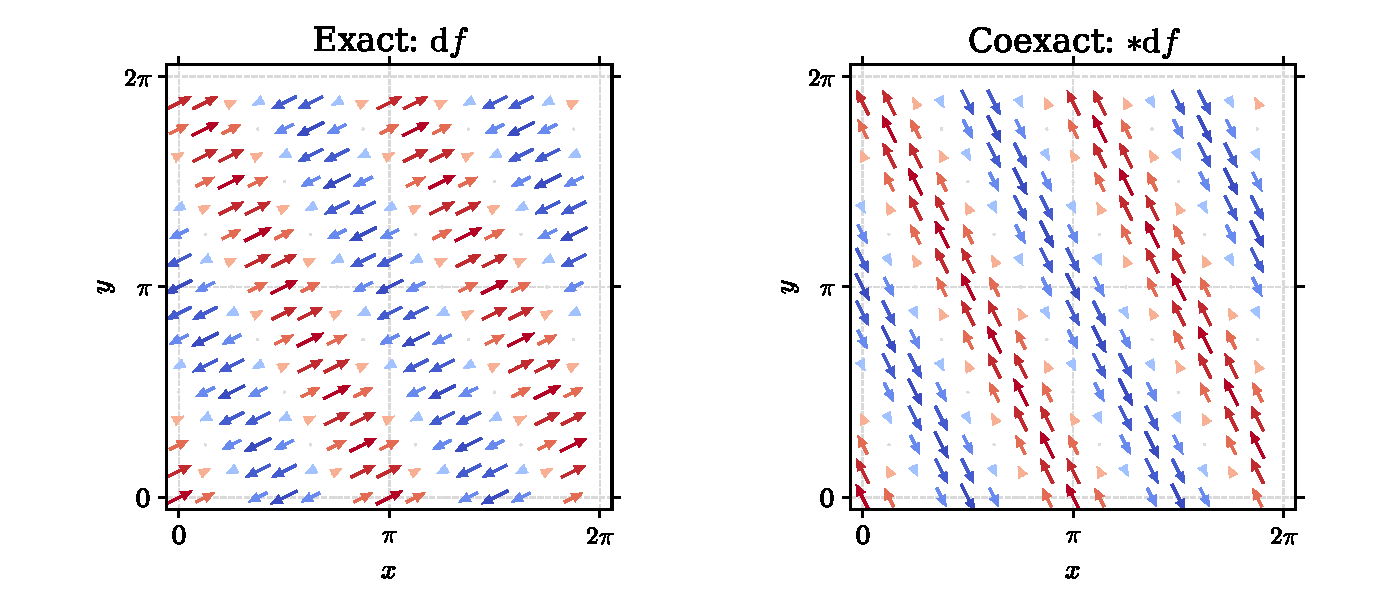
\includegraphics[width=.93\linewidth]{content/MathSkills/figures/geometry-highspin/torus_hodge_vector_modes.pdf}
\caption{\cref{eq:ghs-r9-torus-hodge-sample} 的恰当与余恰当一形式，在环面基本方域上的矢量场箭头。红色表示 $\cos(2x+y)>0$、蓝色表示 $\cos(2x+y)<0$，颜色强度反映其绝对值，两种模式的箭头方向始终正交；边界应按周期识别，不能把图中方域的四条边视为真实物理边界。}\label{fig:ghs-r9-hodge-vector-modes}
\end{figure}

图中的两组箭头采用相同的矢量幅度标尺，箭头长度正比于局部 $|\cos(2x+y)|$，方向和颜色共同标示符号；严格的模态范数仍应使用 $\int_{T^2}|\alpha|^2\dd\mu$。当背景是任意闭定向曲面 $\Sigma$ 时，Hodge 定理仍给出 $\alpha=\dd f+*\dd g+h$，但 $h$ 的维数改为 $2\operatorname{genus}(\Sigma)$，而且不再有简单的整数平面波标签。对有边界的曲面，还必须指定绝对或相对 Hodge 边界条件，才能谈正交分解与零模维数。

\subsection{Hodge、粗拉普拉斯与规范场边界变分}

外微分的幂零关系与联络的曲率作用共同确定一形式场方程，但二者承担不同的约束。

局部张量表示确定了场的分量，但没有确定哪些分量可以独立传播。对带规范冗余的场，还必须把几何上的微分恒等式与动力学约束同时处理。

标量场的谱只需要 $-\Delta$；带自旋的场却生活在非平凡向量丛中，微分算子必须体现联络及曲率。即使是自旋一，也存在至少两种常用的 拉普拉斯算子。若没有弄清楚两者的差别，就容易错误地把普通函数的球谐谱推广成矢量或张量谱。

在定向黎曼流形上，令 $\Omega^p(M)$ 是光滑 $p$ 形式空间，外微分 $\dd:\Omega^p\to\Omega^{p+1}$ 满足 $\dd^2=0$。取 Hodge 星算子 $*$ 与 $L^2$ 内积，外微分的形式伴随记为 $\delta$。这里 $\Delta_H$ 非负；前面的散度型标量算子 $\Delta_g=\operatorname{div}\operatorname{grad}$ 非正，两者在标量上满足 $\Delta_H=-\Delta_g$。在无边界紧致流形上有
\begin{equation}\label{eq:ghs-hodge-laplacian}
 \Delta_{\rm H}=\dd\delta+\delta\dd.
\end{equation}
$\Delta_{\rm H}$ 在 $p$ 形式上非负，因为
$\langle\Delta_{\rm H}\omega,\omega\rangle
 =\norm{\dd\omega}^2+\norm{\delta\omega}^2$。边界存在时这个公式还会出现边界项，故必须补充绝对或相对边界条件。

\begin{theorem}[Hodge 分解]
\label{thm:ghs-hodge-decomposition}
在紧致、无边界、光滑定向黎曼流形上，$L^2$ 的 $p$ 形式有正交分解
\begin{equation}\label{eq:ghs-hodge-direct-sum}
 L^2\Omega^p=\overline{\operatorname{im}\dd}
 \oplus\overline{\operatorname{im}\delta}\oplus\ker\Delta_{\rm H}.
\end{equation}
每个 de Rham 上同调类有唯一调和代表，故 $\dim\ker\Delta_{\rm H}=b_p(M)$，是拓扑不变量。
\end{theorem}
\begin{proof}
$\Delta_{\rm H}$ 是椭圆非负自伴算子，紧致性使其零本征空间有限维，且 Hilbert 空间按核与正谱正交分解。对正谱部分设 $G=\Delta_{\rm H}^{-1}$，则
\[
 \omega=\mathcal H\omega+\Delta_{\rm H}G(1-\mathcal H)\omega
 =\mathcal H\omega+\dd\delta G\omega+\delta\dd G\omega,
\]
$\mathcal H$ 是调和投影。$\dd^2=\delta^2=0$ 和积分分部说明后两个子空间正交；调和形式与它们也正交。若 $\omega$ 闭合，则 $\dd\omega=0$，上式中的余微分项为零，剩下 $\omega=\mathcal H\omega+\dd\alpha$，说明每个闭形式与唯一的调和形式同调。调和且恰当的形式由范数恒等式只能为零，所以代表唯一。
\end{proof}

这个结论对规范场特别重要：零模个数可以由空间拓扑决定，而不由局域曲率常数决定。例如环面上的一形式具有非平凡调和模式，二球上的一般一形式却没有相同的同调零模结构。

联络导出粗 拉普拉斯算子 $\nabla^*\nabla$。对一形式 $\omega_a$，Weitzenböck 恒等式为
\begin{equation}\label{eq:ghs-weitzenbock-one-form}
 (\Delta_{\rm H}\omega)_a=(\nabla^*\nabla\omega)_a
 +\operatorname{Ric}_a{}^b\omega_b.
\end{equation}
它表明曲率以代数势项的形式改变了自旋一的传播算子。对高阶张量也存在相应曲率作用，但不能只用标量曲率 $\mathcal R$ 乘单位矩阵代替全部 Riemann 张量缩并。

\begin{proof}[证明（一形式曲率项的计算）]
对一形式展开协变导数，并交换指标，可核对曲率项的系数。
取 $\delta\omega=-\nabla^a\omega_a$，则
\begin{align*}
(\dd\delta\omega)_b&=-\nabla_b\nabla^a\omega_a,\\
(\delta\dd\omega)_b&=-\nabla^a(\nabla_a\omega_b-\nabla_b\omega_a)\\
&=-\nabla^a\nabla_a\omega_b+\nabla^a\nabla_b\omega_a.
\end{align*}
相加后得到 $-\nabla^a\nabla_a\omega_b+[\nabla^a,\nabla_b]\omega_a$。按照前文固定的曲率约定，该对易项收缩为 $\operatorname{Ric}_b{}^a\omega_a$，于是得 \cref{eq:ghs-weitzenbock-one-form}。这是带自旋算子与标量 拉普拉斯算子的第一个明确差异。

\end{proof}

考虑 $U(1)$ 规范场 $A\in\Omega^1(M)$，曲率 $F=\dd A$，作用量 $\mathscr I[A]=\frac14\int F_{ab}F^{ab}\dd\mu_g=\frac12\norm{\dd A}^2$。规范变换 $A\mapsto A+\dd\alpha$ 不改变 $F$。在 Lorenz 型规范 $\delta A=0$ 下，形式动力学算子与 $\Delta_{\rm H}$ 密切相关。然而零模可能包括精确形式的纯规范方向，以及非精确调和一形式的全局模态；二者必须区别商掉。

若区域有边界，允许的 $\alpha$ 是在边界消失还是可取非零值，直接决定边界荷与 Hilbert 空间分解。不能仅由局域的自旋一张量表示得出规范场全部物理自由度。高自旋规范场也存在类似的约束、迹条件与背景曲率一致性问题。

对对称二张量 $h_{ab}$，取四指标排列 $R_{abcd}=g(R(e_a,e_b)e_c,e_d)$，并记 $R_a{}^c=\operatorname{Ric}_a{}^c$。可以构造一种二阶椭圆算子，其主符号部分是 $-\nabla^2h_{ab}$，曲率作用为
\begin{equation}\label{eq:ghs-lichnerowicz-two-tensor}
 (\Delta_{\rm L}h)_{ab}=-\nabla^c\nabla_ch_{ab}
 +R_a{}^ch_{cb}+R_b{}^ch_{ac}+2R_{acbd}h^{cd}.
\end{equation}
这里的四指标顺序与前面的 $R(X,Y,Z,W)$ 相同；若先降低 $R^a{}_{bcd}$ 的首指标，所得四指标张量等于本式 $R_{abcd}$ 的负值，曲率项便写成常见的 $-2$ 形式。
\begin{proof}[证明（度量张量的零模核对）]
由度规相容性，$\nabla g=0$。由 Ricci 定义与曲率反对称性，
\[
 g^{cd}R_{acbd}=-\operatorname{Ric}_{ab}.
\]
因此取 $h=g$ 时
\[
 (\Delta_{\rm L}g)_{ab}
 =0+\operatorname{Ric}_{ab}+\operatorname{Ric}_{ab}
 +2(-\operatorname{Ric}_{ab})=0.
\]
常截面曲率 $k$ 的直接代入也给出 $R_{acbd}=k(g_{cb}g_{ad}-g_{ab}g_{cd})$，故其收缩为 $-(d-1)kg_{ab}$，与同一 Ricci 定义相符。
\end{proof}
该算子经常出现在 Einstein 方程的线性化、引力子涨落与相关规范固定问题中。它与单独作用于每个分量的标量 拉普拉斯算子 不是同一个算子。

对于更高阶对称无迹张量，二阶算子的可能曲率修正更多；若还要求规范不变性、幺正性和正确约束传播，允许的背景与耦合受到额外限制。这说明“空间任意”与“自旋任意”是两个独立的推广目标，不能在不增加物理假设的情况下同时任意化。

前面的高自旋微分算子涉及协变导数对易子，但对自旋一场还存在更强的结构：规范变换并不要求曲率消失，它直接来自外微分的恒等式 $\dd^2=0$。这一事实提供了区分“曲率使平直表达式失效”和“曲率破坏规范对称性”的一个可完全算通的例子。

先在无边界紧致定向黎曼流形上讨论欧氏二次型。令实一形式 $A=A_a\dd x^a$ 为规范势，$F=\dd A$ 为二形式场强。由于 Levi--Civita 联络无挠，
\begin{equation}\label{eq:ghs-r9-maxwell-fieldstrength}
 F_{ab}=\nabla_aA_b-\nabla_bA_a
 =\partial_aA_b-\partial_bA_a.
\end{equation}
定义作用量 $S[A]=\tfrac12\int_X F\wedge *F=\tfrac14\int_XF_{ab}F^{ab}\dd\mu_g$。变分时 $\delta F=\dd(\delta A)$，对闭流形积分分部：
\begin{align*}
 \delta S
 &=\int_X\dd(\delta A)\wedge *F
 =\langle F,\dd(\delta A)\rangle_{L^2}\\
 &=\langle\delta F,\delta A\rangle_{L^2}.
\end{align*}
这里最后一个 $\delta$ 在 $\delta A$ 中是变分符号，在 $\delta F$ 中则表示余微分；二者的数学角色不同。Euler--Lagrange 方程为
\begin{equation}\label{eq:ghs-r9-maxwell-coexact-eom}
 \delta\dd A=0.
\end{equation}
对任意光滑标量 $\chi$，取 $A\mapsto A+\dd\chi$，由于 $\dd^2\chi=0$，场强和作用量都不变。这一证明对所有光滑黎曼背景成立，不要求 Ricci 曲率为零。

\begin{proposition}[规范场的一形式 Weitzenbock 恒等式]
\label{prop:ghs-r9-maxwell-weitzenbock}
对一形式 $A$，Hodge 拉普拉斯算子满足
\begin{equation}\label{eq:ghs-r9-maxwell-curvature-term}
 (\dd\delta+\delta\dd)A
 =\nabla^*\nabla A+\operatorname{Ric}(A).
\end{equation}
选取 Lorenz 型规范 $\delta A=0$ 后，自由 Maxwell 方程成为 $\Delta_HA=0$。因此在曲空间直接用粗 拉普拉斯算子 $\nabla^*\nabla$ 代替 $\Delta_H$ 会漏掉 Ricci 项；但该项不是外加的规范对称性破缺项，而是由微分复形决定的几何补偿。
\end{proposition}
\begin{proof}
取正定 Laplace 约定，$\delta A=-\nabla^bA_b$，以及 $F_{ba}=\nabla_bA_a-\nabla_aA_b$。于是
\begin{align*}
 (\delta\dd A)_a
 &=-\nabla^bF_{ba}\\
 &=-\nabla^b\nabla_bA_a+\nabla^b\nabla_aA_b.
\end{align*}
另一方面，$(\dd\delta A)_a=-\nabla_a\nabla^bA_b$，所以
\[
 (\Delta_HA)_a=-\nabla^b\nabla_bA_a
 +[\nabla^b,\nabla_a]A_b.
\]
按本书采用的 Ricci 曲率约定，最后的缩并交换子恰为 $\operatorname{Ric}_a{}^bA_b$。第一项是粗 拉普拉斯算子，这就得到了 \cref{eq:ghs-r9-maxwell-curvature-term}。对 $A=\dd\chi$，还可用 $\Delta_H\dd\chi=\dd\Delta_H\chi$ 检查 Ricci 项准确抵消粗 拉普拉斯算子 与梯度不交换的部分。
\end{proof}

这个推导也解释了矢量球谐中两个容易混用的本征值。单位二球若 $\Delta_HY_{\ell m}=\ell(\ell+1)Y_{\ell m}$，则对 $\ell\ge1$，
\[
 \Delta_H(\dd Y_{\ell m})=\ell(\ell+1)\dd Y_{\ell m},\qquad
 \nabla^*\nabla(\dd Y_{\ell m})=[\ell(\ell+1)-1]\dd Y_{\ell m}.
\]
差值恰是 $S^2$ 的 Ricci 本征值 $1$。在环面上 Ricci 为零，两算子则具有相同本征值。这是上述 Hodge 分解、曲率算子以及表示谱的同一个交叉检验，而不是三个互不相干的公式。

如果 $X$ 有边界，$\delta$ 是 $\dd$ 的形式伴随时会出现边界配对；选择绝对或相对边界条件不仅影响自伴性，也影响允许的规范参数与调和零模。即使无边界，零模 $h$ 满足 $\dd h=\delta h=0$ 时仍可出现在 $A$ 中，且不一定是全局的 $\dd\chi$。例如环面上的 $\dd x,\dd y$ 对应不可用单值周期规范函数消去的平坦连接；在耦合带电场时，还需进一步考察它们的整体 holonomy。

将作用量分部积分时保留边界项，可直接得到相应的条件。
设 $X$ 有光滑边界，$\mathbf n$ 为外法向。对紧支于边界附近但边界取值不一定为零的变分，Stokes 定理给出
\[
 \int_X\langle F,\dd(\delta A)\rangle\dd\mu
 =\int_X\langle\delta F,\delta A\rangle\dd\mu
 +\int_{\partial X}\mathbf n^aF_{ab}\,\delta A^b\dd\mu_{\partial X}.
\]
因此固定切向规范势（Dirichlet 型）时边界变分消失；若允许边界 $A$ 自由变化，则自然条件是相应切向分量的 $\mathbf n^aF_{ab}=0$。一般相对/绝对 Hodge 条件还需同时约束规范固定算子的域，不能只规定 $F$ 的一个分量便宣称椭圆自伴问题已经完全确定。边界上的规范变换还可能成为真实的边缘自由度，因而与无边界的情形存在物理差别。


\section{Killing 流与 Hodge 算子的相容性}

Killing 流保持 $g$。因为它从恒等映射连续生成，在局部还保持既定定向，所以同时保持 $\operatorname{vol}_g$。由 Hodge 星的刻画\eqnrefs{eq:math-dg-hodge-star-characterization}可知
\[
\Phi_t^*(*\alpha)=*(\Phi_t^*\alpha).
\]
对 $t=0$ 求导得到
\begin{equation*}[\mathcal L_X,*]=0.
\end{equation*}
再结合 $[\mathcal L_X,\dd]=0$，立即得到
\begin{equation*}[\mathcal L_X,\delta]=0,
\qquad
[\mathcal L_X,\Delta]=0.
\end{equation*}
因此 Hodge 拉普拉斯算子 的每个特征空间都在 Killing 对称下保持。几何对称与谱分解并不是两套独立技巧：它们可以在同一个不变子空间分解中同时使用。
Killing 方程和 Hodge 理论分别控制对称性与微分形式的分解。以下从度量内积与体积形式直接构造星算子、余微分和守恒量。

\section{等距流、Killing 场与守恒量}

有了联络和度量，便能严格表达“空间沿某方向移动后看起来不变”。
设向量场 \(K\) 的局部流为 \(\Phi_t\)：从点 \(p\) 出发，
曲线 \(t\mapsto\Phi_t(p)\) 满足
\(\frac{\dd}{\dd t}\Phi_t(p)=K_{\Phi_t(p)}\)、\(\Phi_0(p)=p\)。
如果流把度量保持不变，即
\(g_{\Phi_t(p)}(\dd\Phi_t X,\dd\Phi_t Y)=g_p(X,Y)\)，
就称 \(\Phi_t\) 为局部等距流。

\begin{definition}[Lie 导数与 Killing 场]
度量沿 \(K\) 的 Lie 导数定义为
\[
(\mathcal L_Kg)_p(X,Y)
=\left.\frac{\dd}{\dd t}\right|_{t=0}
(\Phi_t^*g)_p(X,Y).
\]
若 \(\mathcal L_Kg=0\)，称 \(K\) 为 Killing 场。
\end{definition}

这里 \(\Phi_t^*g\) 表示先用微分 \(\dd\Phi_t\)
把 \(p\) 处两个向量推到 \(\Phi_t(p)\)，再在那里计算 \(g\)。
所以定义不是“直接微分不同点的矩阵”，而是先把不同点的双线性型
拉回同一切空间再比较。

\begin{proposition}[Killing 方程]
对 Levi--Civita 联络，\(K\) 是 Killing 场当且仅当
\[
g(\nabla_XK,Y)+g(X,\nabla_YK)=0
\quad\text{对所有 }X,Y.
\]
在坐标中这等价于
\(\nabla_\mu K_\nu+\nabla_\nu K_\mu=0\)。
\end{proposition}
\begin{proof}
从流的定义对 \(t\) 求导，或在一张坐标图中直接对
\(g_{kl}(\Phi_t(x))\partial_i\Phi_t^k\partial_j\Phi_t^l\)
求导，得到
\[
(\mathcal L_Kg)(X,Y)
=K[g(X,Y)]-g([K,X],Y)-g(X,[K,Y]).
\]
度量相容性给
\(K[g(X,Y)]=g(\nabla_KX,Y)+g(X,\nabla_KY)\)。
无挠性给 \([K,X]=\nabla_KX-\nabla_XK\)，对 \(Y\) 亦然。
代入并约去 \(\nabla_KX,\nabla_KY\) 项，便得到命题中的式子。
\end{proof}

若 \(\gamma(t)\) 是仿射参数测地线，令 \(u=\dot\gamma\)，
则 \(\nabla_uu=0\)。因此
\[
\frac{\dd}{\dd t}g(K,u)
=g(\nabla_uK,u)+g(K,\nabla_uu)=0.
\]
第一项是 Killing 方程取 \(X=Y=u\) 的一半，第二项由
测地线方程消失。这给出守恒量 \(g(K,u)\)。
例如欧氏平面中 \(K=\partial_x\) 产生平移，
\(g(K,u)=\dot x\) 守恒；\(K=-y\partial_x+x\partial_y\)
产生旋转，\(g(K,u)=x\dot y-y\dot x\) 守恒。
由此可见“对称性给守恒量”不是额外的口号，而是度量相容性
与 Killing 方程的直接推论。


\par
\begin{workedexample}
对单位球面度量
\(g=\dd\vartheta^2+\sin^2\vartheta\,\dd\varphi^2\)，
用同一办法计算 \(\Delta_{\rm dR}f\)。
特别检验 \(f=\cos\vartheta\) 满足
\(\Delta_{\rm dR}f=2f\)。
\textbf{解.} 对函数，正号 Hodge--de Rham Laplacian 为负的 Laplace--Beltrami 算子：
\[
\Delta_{\rm dR}f=-\frac1{\sin\vartheta}\partial_\vartheta
(\sin\vartheta\,\partial_\vartheta f)
-\frac1{\sin^2\vartheta}\partial_\varphi^2f.
\]
令 \(f=\cos\vartheta\)，则 \(\partial_\vartheta f=-\sin\vartheta\)，角向散度项为 \(-2\cos\vartheta\)，再乘整体负号得 \(\Delta_{\rm dR}f=2\cos\vartheta=2f\)。
\end{workedexample}
\par
\section{Hodge 对偶从内积与体积形式定义}

上一章已把 \(k\)-形式定义为交替的 \(k\) 重协变张量。
现在先取定向的 \(n\) 维 Riemann 流形，即度量正定；
伪 Riemann 情形的符号稍后单独说明。
在每点选正向正交余标架 \(e^1,\ldots,e^n\)。
体积形式是
\(\mathrm{vol}_g=e^1\wedge\cdots\wedge e^n\)。
若 \(I=(i_1<\cdots<i_k)\)，记
\(e^I=e^{i_1}\wedge\cdots\wedge e^{i_k}\)，
规定这些 \(e^I\) 为 \(\Lambda^kT_p^*M\) 的正交归一基；
这将向量上的度量唯一延拓为 \(k\)-形式上的内积。

\begin{definition}[Hodge 星号]
Hodge 算子 \(*:\Lambda^kT_p^*M\to\Lambda^{n-k}T_p^*M\)
由对任意 \(k\)-形式 \(\alpha,\beta\) 成立的等式
\[
\alpha\wedge *\beta
=\langle\alpha,\beta\rangle\,\mathrm{vol}_g
\]
唯一确定。
\end{definition}

存在性并非显然。对基形式 \(e^I\)，令 \(I^c\) 是补指标组，
定义 \(*e^I=\operatorname{sgn}(I,I^c)e^{I^c}\)，
其中符号由
\(e^I\wedge e^{I^c}
=\operatorname{sgn}(I,I^c)\mathrm{vol}_g\) 决定。
这样 \(e^J\wedge *e^I=\delta_{IJ}\mathrm{vol}_g\)，
再由双线性即可得到定义式。若有另一算子满足同式，
它与此算子之差同所有基 \(e^I\) 作楔积都为零；
补基系数逐一为零，故唯一。

在三维欧氏空间的正向直角坐标下，
\[
*1=\dd x\wedge\dd y\wedge\dd z,
\quad *\dd x=\dd y\wedge\dd z,
\quad *(\dd x\wedge\dd y)=\dd z,
\quad *(\dd x\wedge\dd y\wedge\dd z)=1.
\]
再作一次星号时，两组指标交换经过 \(k(n-k)\) 次换位，因而
\begin{equation}
*^2\alpha=(-1)^{k(n-k)}\alpha
\qquad\bigl(\alpha\in\Lambda^kT_p^*M\bigr).
\label{eq:math-hodge-square}
\end{equation}
这条公式以正定度量为前提。若度量签名有 \(q\) 个负方向，
在常用的正向伪正交基约定下还要乘 \((-1)^q\)；
因此只说 \(*^2=\pm1\) 而不说明维数、形式次数和签名是不完整的。


\par
\begin{workedexample}
在二维欧氏空间的正向坐标中求 \(*\dd x\) 与 \(*\dd y\)，
并直接检验 \cref{eq:math-hodge-square} 对一形式给 \(*^2=-1\)。
\textbf{解.} 在正向正交余标架 \((\dd x,\dd y)\) 下，定义式给
\[
*\dd x=\dd y,\qquad *\dd y=-\dd x.
\]
因此 \(*^2\dd x=-\dd x\)、\(*^2\dd y=-\dd y\)，与 \(k=1,n=2\) 时 \((-1)^{k(n-k)}=-1\) 一致。
\end{workedexample}
\par
\section{余微分与最熟悉的 Laplace 算子}

对紧支撑的形式，定义全空间内积为
\((\alpha,\beta)=\int_M\alpha\wedge *\beta\)。
在无边界流形，或使边界项消失的边界条件下，
外微分 \(\dd:\Omega^{k-1}(M)\to\Omega^k(M)\)
的形式伴随记为 \(\delta:\Omega^k(M)\to\Omega^{k-1}(M)\)，即
\((\dd\alpha,\beta)=(\alpha,\delta\beta)\)。
先取支集包含在一张坐标图内的形式；普通的逐坐标分部积分
使全微分的积分为零。所得等式只涉及点处运算，
故在重叠坐标图上也相同。
注意乘积求导式
\(\dd(\alpha\wedge *\beta)
=\dd\alpha\wedge *\beta+(-1)^{k-1}\alpha\wedge\dd(*\beta)\)，
把全微分项的积分移到另一边，再用星号平方公式，得到
\[
\delta\beta=(-1)^{n(k+1)+1}*\dd *\beta
\quad\text{在 Riemann 度量下}.
\]
边界不消失时，必须额外写出边界积分，不能把形式伴随
直接称为具体 Hilbert 空间算子的伴随。

Laplace--de Rham 算子定义为
\(\Delta_{\rm dR}=\dd\delta+\delta\dd\)。
对零形式即函数 \(f\)，\(\delta f=0\)，故
\(\Delta_{\rm dR}f=\delta\dd f\)。
在欧氏直角坐标中
\(\dd f=\sum_i(\partial_i f)\dd x^i\)，
由上述伴随公式逐项算得
\[
\Delta_{\rm dR}f=-\sum_i\partial_i^2f.
\]
它是分析中非负的 Laplacian \(-\nabla^2\)，与物理教材
常写的 \(\nabla^2\) 只差一个符号约定。
这一例子同时说明，抽象的形式语言最终必须能退回熟悉的偏微分算子。

极坐标不是另一套定义，只是同一算子的另一种写法。
由正交余标架 \(e^1=\dd r,e^2=r\,\dd\varphi\) 有
\(*\dd r=r\,\dd\varphi\)、\(*\dd\varphi=-\dd r/r\)。因此
\[
*\dd f=r(\partial_r f)\,\dd\varphi
-\frac{\partial_\varphi f}{r}\,\dd r,
\quad
\dd*\dd f=\left[\partial_r(r\partial_r f)
+\frac1r\partial_\varphi^2f\right]\dd r\wedge\dd\varphi.
\]
因为体积形式是 \(r\,\dd r\wedge\dd\varphi\)，再用
\(\delta\dd f=-*\dd*\dd f\)，得
\[
\Delta_{\rm dR}f
=-\frac1r\partial_r(r\partial_r f)
-\frac1{r^2}\partial_\varphi^2f.
\]
如果误把 \(\dd\varphi\) 当成单位长度的一形式，
第二项就会少一个 \(r^{-2}\)；余标架的长度不能省略。

电磁学给出另一个直接检验。在三维欧氏空间，先用度量把向量场
\(V\) 变成一形式 \(V^\flat=g(V,\cdot)\)；
把磁场向量 \(\vb{B}\) 记成二形式
\(\mathcal B=*\vb{B}^\flat\)。
按前面的星号表，
\[
\mathcal B=B_x\,\dd y\wedge\dd z
+B_y\,\dd z\wedge\dd x+B_z\,\dd x\wedge\dd y,
\qquad
\dd\mathcal B=(\nabla\cdot\vb{B})\,\dd x\wedge\dd y\wedge\dd z.
\]
对电场一形式 \(\mathcal E=\vb{E}^\flat\) 同样逐项求导，
\(\dd\mathcal E=*(\nabla\times\vb{E})^\flat\)。
所以 Maxwell 的两条无源运动学方程
\(\nabla\cdot\vb{B}=0\)、
\(\nabla\times\vb{E}=-\partial_t\vb{B}\)
恰可写成
\[
\dd\mathcal B=0,
\qquad
\dd\mathcal E+\partial_t\mathcal B=0.
\]
外微分的 \(\dd^2=0\) 还解释了为何若局部写
\(\mathcal B=\dd\mathcal A\)，第一条方程自动成立；
上章的穿孔平面反例同时提醒，局部势的存在不自动保证
它能作为全局单值对象使用。






\section{度量、Killing 与 Hodge 的公式联系}
以下公式采用定向 Riemann 流形的 Hodge 星约定；余微分中的 $k$ 表示它所作用的微分形式次数。Koszul 公式把度量接到联络，Killing 方程则把度量接到流。
\begin{note}[公式之间的联系]
Levi--Civita 联络由 Koszul 公式唯一确定：
\[
\begin{aligned}
2g(\nabla_XY,Z)
={}&Xg(Y,Z)+Yg(Z,X)-Zg(X,Y)\\
&+g([X,Y],Z)-g([Y,Z],X)+g([Z,X],Y).
\end{aligned}
\]
坐标中
\[
\Gamma^k{}_{ij}
=\frac12g^{k\ell}
(\partial_i g_{j\ell}+\partial_j g_{i\ell}-\partial_\ell g_{ij}).
\]
Killing、散度与 Hodge 公式为
\begin{align*}
\mathcal L_Xg&=0,\\
\nabla_iX_j+\nabla_jX_i&=0,\\
\mathcal L_X\operatorname{vol}_g&=(\operatorname{div} X)\operatorname{vol}_g,\\
\operatorname{div} X&=-\delta X^\flat=*\dd*X^\flat,\\
\delta&=(-1)^{n(k+1)+1}*\dd*,\\
\Delta&=\dd\delta+\delta\dd.
\end{align*}
Hodge 分解见\eqnrefs{eq:math-dg-hodge-decomposition}。
\end{note}

\begin{proposition}[Killing 方程的协变表达]
在 Riemann 流形上，\[\mathcal L_Xg=0\quad\Longleftrightarrow\quad\nabla_iX_j+\nabla_jX_i=0.\]对 Killing 场，仿射参数测地线上的 $g(X,\dot\gamma)$ 恒定。
\end{proposition}

\begin{proof}
将 $\mathcal L_Xg$ 的定义用 Levi--Civita 联络改写，利用度量相容性和无挠性消去高阶项，得到一阶方程。

对任意向量场 $Y,Z$，Lie 导数定义给出
\begin{equation*}
 (\mathcal L_Xg)(Y,Z)
 =X[g(Y,Z)]-g([X,Y],Z)-g(Y,[X,Z]).
\end{equation*}
这是 Lie 导数的 Cartan 公式在 $(0,2)$ 张量上的特例：第一项是 $X$ 作用于张量值，后两项扣除 $Y,Z$ 自身被 $X$ 的流推动产生的变化。

Levi--Civita 联络满足 $\nabla g=0$，故
\begin{equation*}
 X[g(Y,Z)]
 =(\nabla_Xg)(Y,Z)+g(\nabla_XY,Z)+g(Y,\nabla_XZ)
 =g(\nabla_XY,Z)+g(Y,\nabla_XZ).
\end{equation*}
度量相容性 $\nabla g=0$ 是 Levi--Civita 联络的两条公理之一，几何意义是"协变微分保持内积"。

$\nabla$ 无挠给出 $[X,Y]=\nabla_XY-\nabla_YX$、$[X,Z]=\nabla_XZ-\nabla_ZX$。代入上面的 Lie 导数定义，
\begin{align*}
 (\mathcal L_Xg)(Y,Z)
 &=g(\nabla_XY,Z)+g(Y,\nabla_XZ)\\
 &\quad -g(\nabla_XY-\nabla_YX,Z)-g(Y,\nabla_XZ-\nabla_ZX).
\end{align*}
无挠性是 Levi--Civita 联络的另一条公理，把 Lie 括号这一纯微分拓扑对象用协变导数表达。

含 $\nabla_XY$ 与 $\nabla_XZ$ 的项相消，留下
\begin{equation*}
 (\mathcal L_Xg)(Y,Z)
 =g(\nabla_YX,Z)+g(Y,\nabla_ZX).
\end{equation*}
此式对任意 $Y,Z$ 成立。注意 $X$ 现在被 $\nabla$ 作用，而不是作用于别人——这是 Killing 方程为一阶 PDE 的关键。

取 $Y=\partial_i$、$Z=\partial_j$，$g(\partial_i,\partial_j)=g_{ij}$，$\nabla_{\partial_i}X$ 的 $j$ 分量为 $\nabla_iX^j$，故
\begin{equation*}
 (\mathcal L_Xg)_{ij}
 =g_{jk}\nabla_iX^k+g_{ik}\nabla_jX^k
 =\nabla_iX_j+\nabla_jX_i.
\end{equation*}
$\mathcal L_Xg=0$ 即给出
\begin{equation}\label{eq:math-dg-synthesis-killing-eq}
\boxed{\nabla_iX_j+\nabla_jX_i=0,}
\end{equation}
即\eqnrefs{eq:math-dg-synthesis-killing-eq}。这是一阶线性 PDE。
沿测地线计算 $\nabla_TT=0$ 及 Killing 方程，得到
\[
\frac{\dd}{\dd s}g(X,T)=g(\nabla_TX,T)=0.
\]
Killing 场的限制是测地线变分的 Jacobi 场。
沿每条径向测地线，$X$ 由 $X(p)$ 与 $\nabla X(p)$ 的初值唯一决定；
Killing 方程又要求 $\nabla X(p)$ 反对称。
故在连通流形上，其第一 jet 的可能维数至多为
$n+\binom n2=n(n+1)/2$，零初值由 Jacobi ODE 的唯一性给出零场。



典型例子。
\begin{itemize}
\item $\RR^n$：平移 $\partial_i$ 与旋转 $x^i\partial_j-x^j\partial_i$ 共 $n+n(n-1)/2=n(n+1)/2$ 个 Killing 场，达到最大维数。
\item $S^n$：$SO(n+1)$ 的 Lie 代数给出 $n(n+1)/2$ 个 Killing 场，对应球面的等距群。
\item $\HH^n$：$SO(n,1)$ 给出 $n(n+1)/2$ 个 Killing 场，双曲空间也是最大对称空间。
\item 一般 Riemann 流形：Killing 场维数 $<n(n+1)/2$，反映对称性的缺失。
\end{itemize}

Killing 场对应度量的连续对称，沿测地线产生守恒量 $J_X=g(X,\dot\gamma)$。在广义相对论中，Killing 场对应时空对称（如稳态时空的时间平移 $\partial_t$ 给出能量守恒、轴对称 $\partial_\phi$ 给出角动量守恒）。Noether 定理在几何语言下即"Killing 场 $\Rightarrow$ 测地线守恒量"。在经典力学中，$n(n+1)/2$ 维最大对称空间对应 $n$ 维自由粒子全部运动积分的存在性。
\end{proof}

\begin{proposition}[Hodge 拉普拉斯的椭圆主符号]
设 $\Delta_H=\dd\delta+\delta\dd$ 作用于 Riemann 流形的 $k$-形式。采用 $\partial_j\mapsto\ii\xi_j$，\[\sigma_2(\Delta_H)(\xi)=|\xi|_g^2\operatorname{id}_{\Lambda^kT_p^*M}.\]故 $\Delta_H$ 椭圆。
\end{proposition}

\begin{proof}
计算 $\Delta=\dd\delta+\delta\dd$ 的二阶主符号。$\dd$ 与 $\delta$ 的一阶主符号分别由外积与插入算子给出，二者复合后用 Cartan 恒等式 $\iota_{\xi^\sharp}(\xi\wedge\cdot)+\xi\wedge\iota_{\xi^\sharp}\cdot=|\xi|^2\,\cdot$ 化为 $|\xi|^2\id()$。

在点 $p$ 处取非零余向量 $\xi\in T_p^*M$。采用 $\partial_j\mapsto \ii\xi_j$ 的主符号约定，外微分与余微分的一阶主符号分别为
\begin{equation*}
\sigma_1(\dd)(\xi)=\ii\,\xi\wedge,
\qquad
\sigma_1(\delta)(\xi)=-\ii\,\iota_{\xi^\sharp}.
\end{equation*}
$\sigma_1(\dd)=\ii\,\xi\wedge$ 来自外微分对一形式 $\alpha$ 给 $\dd\alpha=\partial_i\alpha_j\,\dd x^i\wedge\dd x^j$，主项含一阶导数。$\sigma_1(\delta)=-\ii\,\iota_{\xi^\sharp}$ 来自余微分的 Hodge 星定义与 $\delta=\pm *\dd*$ 中 $*$ 不改变阶数。

因此二阶算子 $\Delta=\dd\delta+\delta\dd$ 的主符号为
\begin{equation*}
\begin{aligned}
\sigma_2(\Delta)(\xi)
&=\sigma_1(\dd)\sigma_1(\delta)+\sigma_1(\delta)\sigma_1(\dd)\\
&=(\ii\,\xi\wedge)(-\ii\,\iota_{\xi^\sharp})
+(-\ii\,\iota_{\xi^\sharp})(\ii\,\xi\wedge)\\
&=(\xi\wedge)\iota_{\xi^\sharp}
+\iota_{\xi^\sharp}(\xi\wedge).
\end{aligned}
\end{equation*}
两个 $\ii$ 与 $-\ii$ 相乘都给 $+1$，符号约定使最终结果为正。

对任意形式 $\alpha$，插入算子与外积满足
\begin{equation*}
\iota_{\xi^\sharp}(\xi\wedge\alpha)
=|\xi|_g^2\alpha
-\xi\wedge\iota_{\xi^\sharp}\alpha.
\end{equation*}
这是 Cartan 公式 $\mathcal L_{\xi^\sharp}=\dd\iota_{\xi^\sharp}+\iota_{\xi^\sharp}\dd$ 在常向量场上的特例，也可直接对单项式 $\alpha=\theta^{i_1}\wedge\cdots\wedge\theta^{i_k}$ 验证：若 $\xi$ 出现在 $\alpha$ 中，插入与外积相继给出 $|\xi|^2$；若不出现，外积先添加该方向，插入再移除，仍给出 $|\xi|^2\alpha$；两种情形都是同一个反对易恒等式。

把 Cartan 恒等式代入主符号表达式，
\begin{equation*}
\iota_{\xi^\sharp}(\xi\wedge\alpha)
+\xi\wedge\iota_{\xi^\sharp}\alpha
=|\xi|_g^2\alpha
-\xi\wedge\iota_{\xi^\sharp}\alpha
+\xi\wedge\iota_{\xi^\sharp}\alpha
=|\xi|_g^2\alpha,
\end{equation*}
两项相消，恰好得到
\begin{equation}\label{eq:math-dg-hodge-principal-symbol}
\boxed{
\sigma_2(\Delta)(\xi)
=|\xi|_g^2\id(\Lambda^kT_p^*M).}
\end{equation}
当 $\xi\neq0$ 时该线性映射可逆，故 $\Delta$ 是椭圆算子。结合\eqnrefs{eq:math-dg-hodge-energy}的非负性与适当自伴定义域，就能调用前面建立的自伴谱理论，而不必把 Hodge 分解当作孤立结论。

典型例子与对比。
\begin{itemize}
\item $\RR^n$ 上 $0$-形式（函数）：$\Delta f=-\sum_i\partial_i^2 f$（本书非负约定），主符号 $|\xi|^2$，正是普通 拉普拉斯算子。
\item $\RR^n$ 上 $1$-形式：$\Delta\alpha_j=-\sum_i\partial_i^2\alpha_j$，每个分量独立满足标量 拉普拉斯算子，主符号仍是 $|\xi|^2\id()$。
\item 一般流形：主符号与 $\RR^n$ 相同，但低阶项含曲率（见 Weitzenböck 公式 $\Delta_H=\nabla^*\nabla+\operatorname{Ric}$），曲率通过低阶项影响谱而非椭圆性。
\end{itemize}

Hodge 拉普拉斯算子 的椭圆性是 Hodge 定理成立的分析基础：椭圆 + 自伴 + 非负 + 紧致流形 $\Rightarrow$ 谱离散且有限维核。在物理中，紧致空间上经过适当规范固定的椭圆线性化具有有限维核；这不能直接推广为全部非线性规范场解空间有限维，以及弦理论中 拉普拉斯算子 谱决定物理态能级。Weitzenböck 公式把椭圆性 + 曲率正性结合，给出 Bochner 消没定理——曲率通过低阶项直接控制核空间维数。
\end{proof}

\begin{theorem}[Green 算子与 Hodge 分解]
在紧致、定向、无边界 Riemann 流形上，每个光滑 $k$-形式唯一分解为三个两两正交分量\[\alpha=\Pi_{\mathcal H,k}\alpha+\dd\delta\mathcal G_k\alpha+\delta\dd\mathcal G_k\alpha.\]每个 de Rham 类有唯一调和代表，两个势本身可不唯一。
\end{theorem}

\begin{proof}
在紧致无边界流形上，限制在 $\Omega^k(M)$ 的椭圆自伴算子记为 $\Delta_k$。它具有离散非负谱，零特征空间就是有限维的 $\mathcal H^k(M)$。记到该零空间的正交投影为 $\Pi_{\mathcal H,k}$，并在其正交补上定义 Green 算子
\[
\mathcal G_k:=\left(\Delta_k\big|_{\mathcal H^k(M)^\perp}\right)^{-1},
\qquad
\mathcal G_k\eta=0\quad(\eta\in\mathcal H^k(M)).
\]
于是谱分解给出精确算子恒等式
\[
I=\Pi_{\mathcal H,k}+\Delta_k\mathcal G_k.
\]
对任意 $\alpha\in\Omega^k(M)$，直接展开 $\Delta_k=\dd\delta+\delta\dd$ 得
\[
\begin{aligned}
\alpha
&=\Pi_{\mathcal H,k}\alpha+\Delta_k\mathcal G_k\alpha\\
&=\Pi_{\mathcal H,k}\alpha
+\dd\delta\mathcal G_k\alpha
+\delta\dd\mathcal G_k\alpha.
\end{aligned}
\]
令
\[
\alpha_{\mathcal H}=\Pi_{\mathcal H,k}\alpha,
\qquad
\beta=\delta\mathcal G_k\alpha,
\qquad
\gamma=\dd\mathcal G_k\alpha,
\]
便得到\eqnrefs{eq:math-dg-hodge-decomposition}。

三个分量两两正交。例如
\[
(\dd\beta,\delta\gamma)
=(\dd^2\beta,\gamma)=0,
\]
而对 调和 分量 $\alpha_{\mathcal H}$，由 $\dd\alpha_{\mathcal H}=\delta\alpha_{\mathcal H}=0$，
\[
(\dd\beta,\alpha_{\mathcal H})=(\beta,\delta\alpha_{\mathcal H})=0,
\qquad
(\delta\gamma,\alpha_{\mathcal H})=(\gamma,\dd\alpha_{\mathcal H})=0.
\]
因此三项本身唯一。若只改变 $\beta$ 为 $\beta+\zeta$ 且 $\dd\zeta=0$，精确 分量不变，所以势并不唯一；$\gamma$ 同理。

最后证明调和代表与 de Rham 上同调一一对应。调和形式由\eqnrefs{eq:math-dg-harmonic-closed-coclosed}必为闭形式，故定义上同调类。若 $\eta_1-\eta_2=\dd\zeta$ 且 $\eta_1,\eta_2$ 都 调和，则
\[
\|\eta_1-\eta_2\|^2
=(\eta_1-\eta_2,\dd\zeta)
=(\delta(\eta_1-\eta_2),\zeta)=0,
\]
所以同一上同调类至多一个 调和 代表。另一方面若 $\alpha$ 闭，Hodge 分解给出
\[
\alpha=\dd\beta+\delta\gamma+\alpha_{\mathcal H}.
\]
对两边作用 $\dd$，得到 $\dd\delta\gamma=0$。于是
\[
\|\delta\gamma\|^2
=(\gamma,\dd\delta\gamma)=0,
\]
故 $\delta\gamma=0$，从而 $[\alpha]=[\alpha_{\mathcal H}]$。存在性成立。
\end{proof}

\begin{theorem}[实 de Rham 上同调的 Poincaré 对偶]
设 $M^n$ 紧致、定向、无边界。配对\[H^k_{\mathrm{dR}}(M;\RR)\times H^{n-k}_{\mathrm{dR}}(M;\RR)\to\RR,\qquad([\alpha],[\beta])\mapsto\int_M\alpha\wedge\beta\]良定义且非退化，故 $b_k=b_{n-k}$。
\end{theorem}

\begin{proof}
先验证\eqnrefs{eq:math-dg-poincare-pairing}只依赖上同调类。若 $\alpha\mapsto\alpha+\dd\eta$ 且 $\beta$ 闭，则由 $\dd\beta=0$ 及外微分 Leibniz 律
\[
\dd(\eta\wedge\beta)
=\dd\eta\wedge\beta+(-1)^{\deg\eta}\eta\wedge\dd\beta
=\dd\eta\wedge\beta,
\]
故由 Stokes 定理及 $\partial M=\varnothing$，
\[
\int_M\dd\eta\wedge\beta
=\int_M\dd(\eta\wedge\beta)
=\int_{\partial M}\eta\wedge\beta
=0.
\]
对 $\beta$ 的 精确 改变 $\beta\mapsto\beta+\dd\zeta$ 同理，因 $\alpha$ 闭且
\[
\dd(\alpha\wedge\zeta)
=\dd\alpha\wedge\zeta+(-1)^{\deg\alpha}\alpha\wedge\dd\zeta
=(-1)^{\deg\alpha}\alpha\wedge\dd\zeta,
\]
故
\[
\int_M\alpha\wedge\dd\zeta
=(-1)^k\int_M\dd(\alpha\wedge\zeta)=0.
\]
因此配对在上同调上良定。

现在取非零上同调类 $[\alpha]\neq0$，并令 $h$ 为其唯一调和代表元，即 $\Delta h=0$。由\eqnrefs{eq:math-dg-hodge-star-harmonic-isomorphism}，Hodge 星保持 调和 性，故 $*h$ 也是 调和，因此定义一个 $(n-k)$ 次上同调类
\[
[*h]\in H^{n-k}_{\mathrm{dR}}(M).
\]
于是由 Hodge 星的定义\eqnrefs{eq:math-dg-hodge-star-characterization}，
\begin{align*}
\int_M h\wedge *h
&=\int_M \langle h,h\rangle_g\,\operatorname{vol}_g\\
&=\int_M |h|_g^2\,\operatorname{vol}_g\\
&=\|h\|_{L^2}^2.
\end{align*}
由 $[\alpha]\neq0$ 故 $h\neq0$，从而
\[
\|h\|_{L^2}^2>0.
\]
所以 $[\alpha]$ 与 $[*h]$ 配对非零，不可能与所有 $H^{n-k}_{\mathrm{dR}}(M)$ 元素配对为零。反向非退化性由 $**h=(-1)^{k(n-k)}h$ 完全相同地得到：对非零 $[\beta]\in H^{n-k}_{\mathrm{dR}}(M)$，取其 调和 代表元 $k$，则
\[
\int_M k\wedge *k=\|k\|_{L^2}^2>0,
\]
故 $[\beta]$ 与 $[*k]\in H^k_{\mathrm{dR}}(M)$ 配对非零。因此配对非退化，而有限维向量空间之间的非退化配对立刻给出
\[
\dim H^k_{\mathrm{dR}}(M)
=\dim H^{n-k}_{\mathrm{dR}}(M).
\]

紧曲面 $\Sigma_g$（亏格 $g$）满足 $b_0=b_2=1$、$b_1=2g$，因而 $b_k=b_{2-k}$ 逐次成立；中间次数 $k=1$ 是自对偶的。紧 3-流形如 $T^3$ 则有 $b_0=b_3=1$、$b_1=b_2=3$。Poincaré 对偶不仅是维数等式，还给出上积配对 $H^k\times H^{n-k}\to H^n\cong\mathbb R$ 的非退化性——这是相交理论的基础：$k$-形式与 $(n-k)$-形式的上积对应对偶子流形的相交数。
\end{proof}

\begin{proposition}[一形式的 Weitzenböck 公式]
对 Riemann 流形上的光滑一形式，\[(\Delta_H\alpha)_j=(\nabla^*\nabla\alpha)_j+\operatorname{Ric}_j{}^k\alpha_k.\]在紧致无边界且 $\operatorname{Ric}>0$ 时，每个调和一形式为零。
\end{proposition}

\begin{proof}
对 $1$-形式 $\alpha$，分别计算 $\delta\dd\alpha$ 与 $\dd\delta\alpha$ 的分量，相加后把"协变导数交换子"识别为 Ricci 曲率，得到 $\Delta_H=\nabla^*\nabla+\operatorname{Ric}$。

对 $1$-形式 $\alpha=\alpha_j\dd x^j$，采用
\begin{equation*}
(\dd\alpha)_{ij}
=\nabla_i\alpha_j-\nabla_j\alpha_i,
\qquad
\delta\alpha=-\nabla^i\alpha_i.
\end{equation*}
第一个是外微分的协变分量形式（无挠使 Christoffel 项相消），第二个是余微分的分量约定（散度的负号来自本书非负 拉普拉斯算子 约定）。

把 $\dd\alpha$ 视为 $2$-形式再作用 $\delta$：
\begin{equation*}
(\delta\dd\alpha)_j
=-\nabla^i(\dd\alpha)_{ij}
=-\nabla^i(\nabla_i\alpha_j-\nabla_j\alpha_i)
=-\nabla^i\nabla_i\alpha_j+\nabla^i\nabla_j\alpha_i.
\end{equation*}
第一项是非负约定的联络拉普拉斯 $\nabla^*\nabla$ 的主项，第二项保留待与 $\dd\delta\alpha$ 中的对应项合并。


\begin{equation*}
(\dd\delta\alpha)_j
=\nabla_j(\delta\alpha)
=-\nabla_j\nabla^i\alpha_i.
\end{equation*}
此处用了 $1$-形式 $\delta\alpha$ 的外微分分量公式 $(\dd f)_j=\nabla_j f$。

相加得到
\begin{equation*}
(\Delta_H\alpha)_j
=(\delta\dd\alpha+\dd\delta\alpha)_j
=-\nabla^i\nabla_i\alpha_j
+\nabla^i\nabla_j\alpha_i
-\nabla_j\nabla^i\alpha_i.
\end{equation*}
最后两项正是协变导数交换子。对协变 $1$-张量，
\begin{equation*}
(\nabla^i\nabla_j-\nabla_j\nabla^i)\alpha_i
=\operatorname{Ric}_j{}^k\alpha_k
\end{equation*}
（符号与本书前面的 Riemann 曲率 约定 相容）。这一识别来自 Riemann 曲率的分量定义 $[\nabla_a,\nabla_b]X^c=R^c{}_{dab}X^d$，对协变指标取 迹 给 Ricci：$R^i{}_{j i k}\alpha^k=\operatorname{Ric}_{jk}\alpha^k$。

另一方面，正规坐标中
\begin{equation*}
(\nabla^*\nabla\alpha)_j
=-\nabla^i\nabla_i\alpha_j
\end{equation*}
在基点成立，张量性使其全局成立，因此得到\eqnrefs{eq:math-dg-weitzenbock-oneform}。

典型例子与应用。
\begin{itemize}
\item $\RR^n$：$\operatorname{Ric}=0$，$\Delta_H=\nabla^*\nabla=-\sum_i\partial_i^2$，每个分量独立满足标量 拉普拉斯算子。
\item $S^n$（$n\ge2$，Ric $=(n-1)g$）：$\Delta_H=\nabla^*\nabla+(n-1)$。调和 $1$-形式满足 $\nabla^*\nabla\alpha=-(n-1)\alpha$，但 $\nabla^*\nabla$ 非负，故 $\alpha=0$，即 $H^1(S^n)=0$（$n\ge2$）。
\item 紧致流形 $\operatorname{Ric}>0$：Bochner 消没定理给 $H^1(M)=0$，结合 Bonnet--Myers 定理（$\operatorname{Ric}\ge(n-1)k>0$ $\Rightarrow$ 直径 $\le\pi/\sqrt{k}$）说明正 Ricci 曲率强烈限制流形拓扑。
\end{itemize}

对紧致、无边界的 Spin 流形，未扭曲 Dirac 算子满足
$D^2=\nabla^*\nabla+\mathrm{Scal}/4$。
若 $\mathrm{Scal}>0$，能量恒等式推出 $\ker D=0$。
在偶数维，进一步结合分次算子 $D^+$ 的 Atiyah--Singer 指标公式，
得到 $\operatorname{ind}(D^+)=\hat A(M)=0$。
若加入非平坦扭曲丛，平方中还有丛曲率项，不能只凭正标量曲率断言核为零。
热核的分次迹 $\operatorname{Str}(e^{-tD^2})$ 将局部曲率项与全局指标联系起来，
这一联系将在旋量章节的 Lichnerowicz 公式中继续展开。
\end{proof}

\begin{theorem}[Lichnerowicz 谱隙下界]
设 $(M^n,g)$ 紧致、连通、无边界，$n\ge2$，$\operatorname{Ric}\ge(n-1)kg$、$k>0$。非负函数拉普拉斯 $\Delta=-\Delta_{\mathrm{LB}}$ 的第一正本征值满足 $\lambda_1\ge nk$。
\end{theorem}

\begin{proof}
设 $(M^n,g)$ 紧致无边界，$\operatorname{Ric}\ge(n-1)kg$（$k>0$），$\Delta f=\lambda_1 f$（第一非零本征函数）。

对本征函数积分\eqnrefs{eq:math-dg-bochner-function}。紧致无边界时 Stokes 定理给出 $\int_M\Delta|\nabla f|^2\operatorname{vol}_g=0$（边界项消失），于是
\begin{equation*}
 0
 =\lambda_1\int_M|\nabla f|^2\operatorname{vol}_g
 -\int_M|\nabla^2f|^2\operatorname{vol}_g
 -\int_M\operatorname{Ric}(\nabla f,\nabla f)\operatorname{vol}_g.
\end{equation*}

由 Green 公式，
\begin{equation*}
 \int_M|\nabla f|^2\operatorname{vol}_g
 =\int_M f\,\Delta f\,\operatorname{vol}_g
 =\lambda_1\int_M f^2\operatorname{vol}_g.
\end{equation*}

由 Cauchy--Schwarz 不等式对 Hessian 的迹，
\begin{equation*}
 |\nabla^2 f|^2\ge\frac{1}{n}(\tr\nabla^2f)^2
 =\frac{1}{n}(\Delta f)^2
 =\frac{\lambda_1^2}{n}f^2.
\end{equation*}
由 Ricci 下界假设，
\begin{equation*}
 \operatorname{Ric}(\nabla f,\nabla f)\ge(n-1)k\,|\nabla f|^2.
\end{equation*}

这里只能在积分以后使用
$\int|\nabla f|^2=\lambda_1\int f^2$，点态恒等式 $|\nabla f|^2=\lambda_1f^2$ 不成立。
将两个下界代入上面的 Bochner 恒等式（移项后右端 $\ge0$）：
\begin{align*}
 0
 &\le \lambda_1^2\int_Mf^2\operatorname{vol}_g
  -\frac{\lambda_1^2}{n}\int_Mf^2\operatorname{vol}_g
  -(n-1)k\lambda_1\int_Mf^2\operatorname{vol}_g\\
 &=\lambda_1\left(\frac{(n-1)\lambda_1}{n}-(n-1)k\right)\int_Mf^2\operatorname{vol}_g\\
 &=(n-1)\lambda_1\left(\frac{\lambda_1}{n}-k\right)\int_Mf^2\operatorname{vol}_g.
\end{align*}

因为 $\lambda_1>0$（非常数本征函数）、$n>1$、$f\not\equiv0$，积分因子为正，故 $\lambda_1/n-k\ge0$，即 $\lambda_1\ge nk$。这就是\eqnrefs{eq:math-dg-lichnerowicz-gap}。

Lichnerowicz 下界与 Bonnet--Myers 直径上界 $\operatorname{diam}(M)\le\pi/\sqrt{k}$ 假设完全相同（$\operatorname{Ric}\ge(n-1)kg$），但结论从"直径有限"变成"拉普拉斯算子 的第一个正本征值远离零"。同一个 Ricci 下界同时约束几何尺度与低频谱。
\end{proof}

\begin{proposition}[Hodge 边界条件的 Green 能量恒等式]
设 $M$ 紧致、定向且有光滑边界。绝对条件 $\iota_\nu\omega=\iota_\nu\dd\omega=0$ 或相对条件 $j^*\omega=j^*\delta\omega=0$ 均推出\[(\Delta_H\omega,\omega)=\|\dd\omega\|^2+\|\delta\omega\|^2.\]调和零模闭且余闭，Hodge 星给出 $\mathcal H_A^k\cong\mathcal H_R^{n-k}$。
\end{proposition}

\begin{proof}
设 $M$ 为紧致、定向的 Riemann 流形，边界光滑，$\nu$ 为外法单位向量。
先对实微分形式计算；复形式在第二槽取共轭，结论相同。
对 $\alpha\in\Omega^{k-1}(M)$、$\beta\in\Omega^k(M)$，外微分乘积规则给出
\[
\dd(\alpha\wedge *\beta)
=\dd\alpha\wedge *\beta+(-1)^{k-1}\alpha\wedge\dd(*\beta).
\]
按正文的余微分约定，第二项积分为 $-(\alpha,\delta\beta)$。
Stokes 定理因而给出
\[
(\dd\alpha,\beta)-(\alpha,\delta\beta)
=\int_{\partial M}j^*(\alpha\wedge *\beta)
=\int_{\partial M}\langle\alpha,\iota_\nu\beta\rangle\,\dd S.
\]
最后一个等号可在正交余标架 $(\nu^\flat,\theta^1,\dots)$ 中验证：
只有 $\beta$ 的法向分量与 $\alpha$ 的切向分量参与边界积分。

对 $\Delta\omega=\delta\dd\omega+\dd\delta\omega$ 分别使用上式，得
\begin{align*}
(\delta\dd\omega,\omega)
&=\|\dd\omega\|^2-
\int_{\partial M}\langle\omega,\iota_\nu\dd\omega\rangle\,\dd S,\\
(\dd\delta\omega,\omega)
&=\|\delta\omega\|^2+
\int_{\partial M}\langle\delta\omega,\iota_\nu\omega\rangle\,\dd S.
\end{align*}
绝对条件 $\iota_\nu\omega=0$、$\iota_\nu\dd\omega=0$
逐项消去边界积分。相对条件 $j^*\omega=0$、$j^*\delta\omega=0$
则消去其中的切向因子。故两种域都满足
\[
(\Delta\omega,\omega)=\|\dd\omega\|^2+\|\delta\omega\|^2.
\]
若 $\Delta\omega=0$，两项非负，必有 $\dd\omega=\delta\omega=0$。
能量恒等式证明非负性和零模的闭、余闭性质；完整自伴性还使用
Hodge--Morrey--Friedrichs 的椭圆边界理论，不能只由一次分部积分宣称已经证明。

Hodge 星的点态恒等式
\[
\iota_\nu(*\omega)=*(\omega\wedge\nu^\flat),\qquad
**\omega=(-1)^{k(n-k)}\omega
\]
说明它交换切向和法向分量。再利用 $\delta*=\pm*\dd$，
绝对条件的两条式子变为 $j^*(*\omega)=0$、$j^*\delta(*\omega)=0$。
因此 $*:\mathcal H_A^k\to\mathcal H_R^{n-k}$ 是同构。

区间上的 $0$-形式使两种条件完全可见：绝对条件为
$f'(0)=f'(1)=0$，相对条件为 $f(0)=f(1)=0$。
$-f''=0$ 的 Neumann 解是常数，而 Dirichlet 解只有零。
相应地，$H^0([0,1])=\RR$、$H^0([0,1],\partial[0,1])=0$。

在乘积平坦度量的圆柱 $S^1\times[0,1]$ 上，$\dd\theta$ 是绝对调和
$1$-形式，$\dd t$ 是相对调和 $1$-形式。两种空间维数都为一，
但选出的代表不同；维数不能被写成必然不同。
圆盘以及半球同胚于闭球 $D^n$，其上同调为
\[
H^k(D^n)=
\begin{cases}\RR,&k=0,\\0,&k>0,\end{cases}
\qquad
H^k(D^n,\partial D^n)=
\begin{cases}\RR,&k=n,\\0,&k\ne n.\end{cases}
\]
特别地 $H^1(D^2,\partial D^2)=0$，非平凡相对类在次数 $2$，
由体积形式代表。半球的普通上同调不能等同于整个球面 $S^n$ 的上同调。
这些结果也可由可缩性、对偶定理与配对长正合列分别核对。

无边界时两种域重合，恢复通常的 Hodge 分解。
非定向的 Möbius 带则需要取向线丛：Hodge 星把普通形式映为取向扭曲的形式，
也可以在可定向二重覆盖上施加正确的奇偶条件，不能忽略该变换的类型。
\end{proof}

